\documentclass[a4paper, 11pt]{article}
\usepackage[utf8]{inputenc}
\usepackage[english]{babel}
\usepackage[utf8]{inputenc}
\usepackage[margin=2.cm]{geometry}
\usepackage{fancyhdr}

\usepackage[T1]{fontenc}
\usepackage{lmodern}

\usepackage{graphicx}
\graphicspath{ {images/} }
\usepackage{pdflscape}


\usepackage{array}

\usepackage{color,array}

\definecolor{mygray}{gray}{0.6} %custom color for text

\usepackage{float}
\usepackage[table,xcdraw]{xcolor}


\usepackage{varwidth} %for lists next to each other

%for subfigure
\usepackage{subcaption}


%Includes "References" in the table of contents
\usepackage[nottoc]{tocbibind}

\usepackage{enumitem}
\setlist{nolistsep}

\fancypagestyle{plain}{%
  \renewcommand{\headrulewidth}{0pt}%
  \fancyhf{}%
  \fancyfoot[L]{\footnotesize Raymond Lochner}
  \fancyfoot[C]{\footnotesize November 2017 - Université libre de Bruxelles}%
  \fancyfoot[R]{\thepage}
}
\pagestyle{plain}

\date{\today}

\begin{document}

\begin{titlepage}
	\centering
	{\scshape\LARGE Université libre de Bruxelles \par}
	\vspace{1cm}
	{\scshape\Large INFO-F-409 - Learning Dynamics\par}
	\vspace{1.5cm}
	{\huge\bfseries {Assignment Two\par}}
	\vspace{2cm}
	{\Large Raymond Lochner - 000443637\par}
	\vspace{0.5cm}
	{\Large raymond.lochner@ulb.ac.be}
	\vfill
	
	\setcounter{tocdepth}{2} %hides subsubsections in TOC
	\tableofcontents

\vfill
% Bottom of the page
	{\large \today \par}
\end{titlepage}

\newpage

\section*{Preliminary information}

Each simulation was being executed 100 times.
For the visualizations:
\begin{itemize}[noitemsep]
  \item Red signifies the action \textit{cooperation}
  \item Blue signifies the action \textit{defection}
\end{itemize}

Graphic displays one specific game, Graph shows information of all games



\section{Part One - Spatial Prisoners Dilemma}

\subsection{Moore Neighborhood}

\newpage


%%%% 4x4
%%%%%%%%%%%%%%%%%%%%%%%%%%%%%%%%%%%%%%%%%
\subsubsection{4x4}
\begin{figure}[H]
\centering
\begin{subfigure}{.16\textwidth}
  \centering
  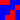
\includegraphics[width=0.9\linewidth]{PRISONERS_DILEMMA_MOORE_4x4_t00}
  \caption{t=0}
\end{subfigure}%
\begin{subfigure}{.16\textwidth}
  \centering
  
\includegraphics[width=0.9\linewidth]{PRISONERS_DILEMMA_MOORE_4x4_t01}
  \caption{t=1}
\end{subfigure}%
\begin{subfigure}{.16\textwidth}
  \centering
  
\includegraphics[width=0.9\linewidth]{PRISONERS_DILEMMA_MOORE_4x4_t05}
  \caption{t=5}
\end{subfigure}%
\begin{subfigure}{.16\textwidth}
  \centering
  
\includegraphics[width=0.9\linewidth]{PRISONERS_DILEMMA_MOORE_4x4_t10}
  \caption{t=10}
\end{subfigure}%
\begin{subfigure}{.16\textwidth}
  \centering
  
\includegraphics[width=0.9\linewidth]{PRISONERS_DILEMMA_MOORE_4x4_t20}
  \caption{t=20}
\end{subfigure}%
\begin{subfigure}{.16\textwidth}
  \centering
  
\includegraphics[width=0.9\linewidth]{PRISONERS_DILEMMA_MOORE_4x4_t50}
  \caption{t=50}
\end{subfigure}
\caption{Prisoners Dilemma, Moore, 4x4}
\end{figure}

\begin{figure}[H]
\begin{subfigure}{.75\textwidth}
	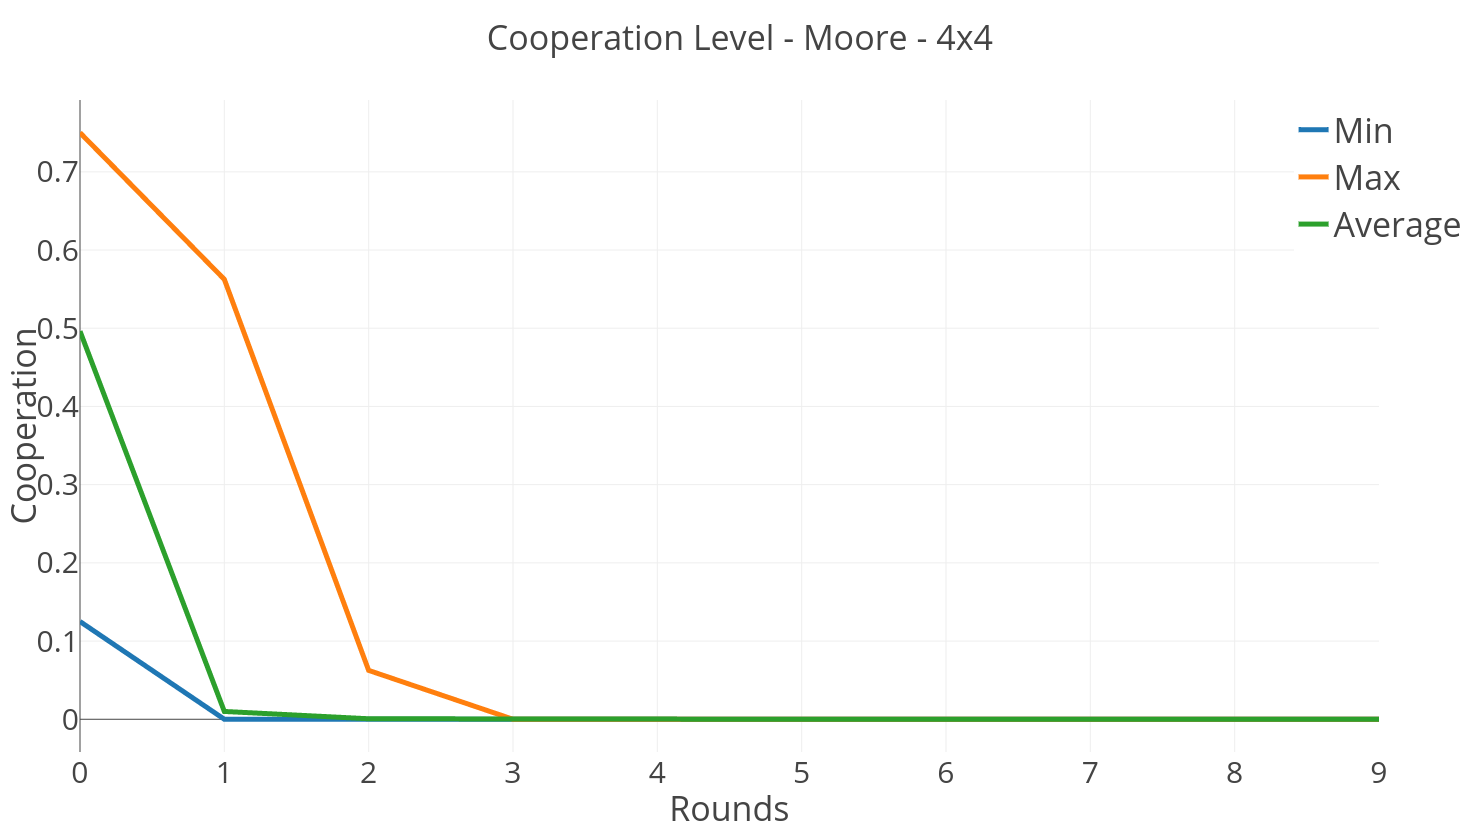
\includegraphics[width=1\linewidth]{PDMoore4x4}
\end{subfigure}

\begin{subfigure}{.75\textwidth}
	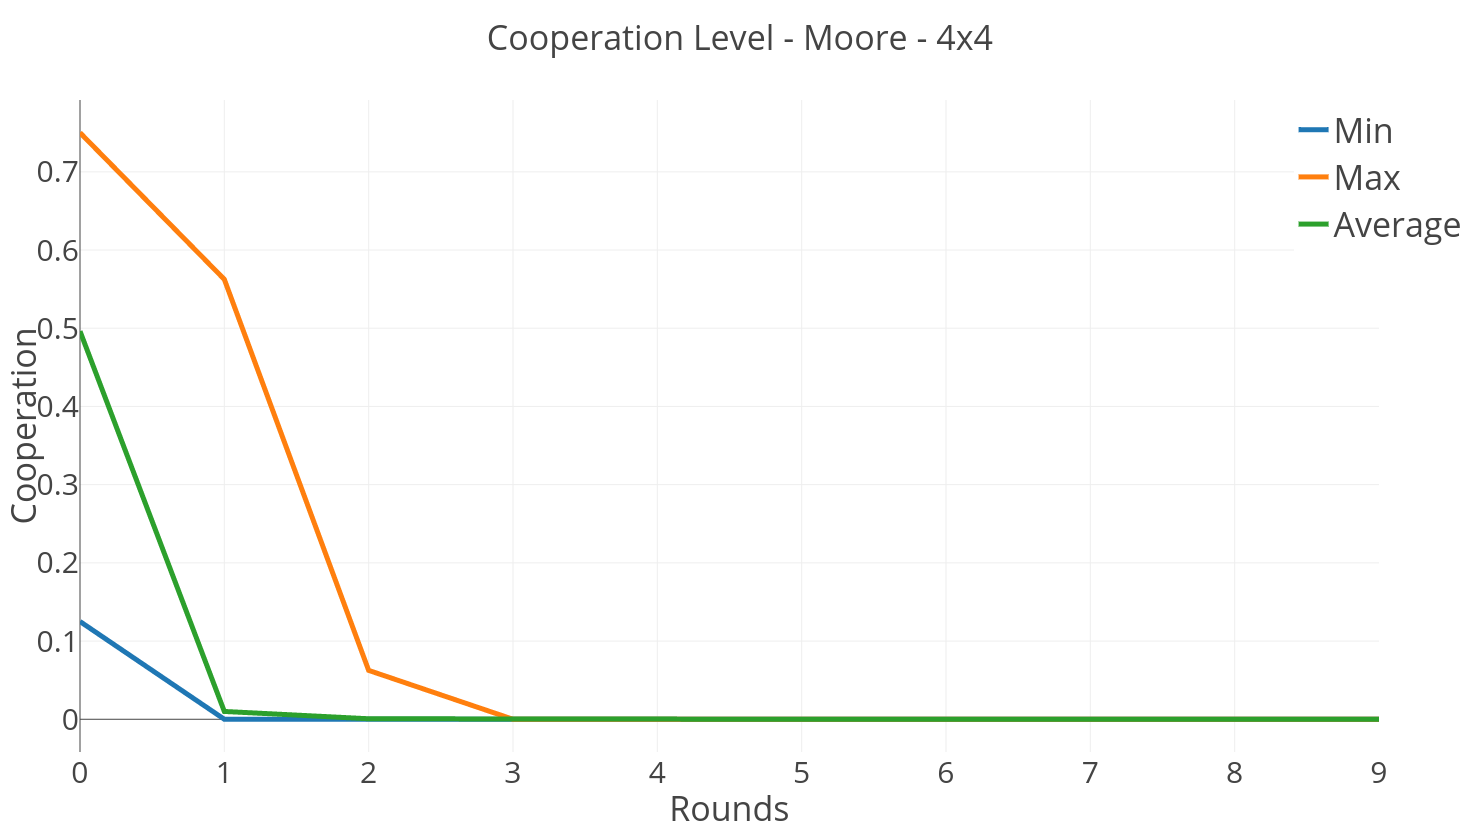
\includegraphics[width=1\linewidth]{PDMoore4x4}
\end{subfigure}

\end{figure}

	From simulating 100 runs we observe that all converge to \textit{defecting}. It is however possible that it converges to a cooperative field, but it requires that we have a sub-matrix of 2x2 with only cooperators and all other players being defectors. This did obviously not happen during one of the simulations.


\newpage

%%%% 8x8
%%%%%%%%%%%%%%%%%%%%%%%%%%%%%%%%%%%%%%%%%
\subsubsection{8x8}
\begin{figure}[H]
\centering
\begin{subfigure}{.16\textwidth}
  \centering
  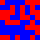
\includegraphics[width=0.9\linewidth]{PRISONERS_DILEMMA_MOORE_8x8_t00}
  \caption{t=0}
\end{subfigure}%
\begin{subfigure}{.16\textwidth}
  \centering
  
\includegraphics[width=0.9\linewidth]{PRISONERS_DILEMMA_MOORE_8x8_t01}
  \caption{t=1}
\end{subfigure}%
\begin{subfigure}{.16\textwidth}
  \centering
  
\includegraphics[width=0.9\linewidth]{PRISONERS_DILEMMA_MOORE_8x8_t05}
  \caption{t=5}
\end{subfigure}%
\begin{subfigure}{.16\textwidth}
  \centering
  
\includegraphics[width=0.9\linewidth]{PRISONERS_DILEMMA_MOORE_8x8_t10}
  \caption{t=10}
\end{subfigure}%
\begin{subfigure}{.16\textwidth}
  \centering
  
\includegraphics[width=0.9\linewidth]{PRISONERS_DILEMMA_MOORE_8x8_t20}
  \caption{t=20}
\end{subfigure}%
\begin{subfigure}{.16\textwidth}
  \centering
  
\includegraphics[width=0.9\linewidth]{PRISONERS_DILEMMA_MOORE_8x8_t50}
  \caption{t=50}
\end{subfigure}
\caption{Prisoners Dilemma, Moore, 8x8}
\end{figure}


\begin{figure}[H]
\begin{subfigure}{.75\textwidth}
	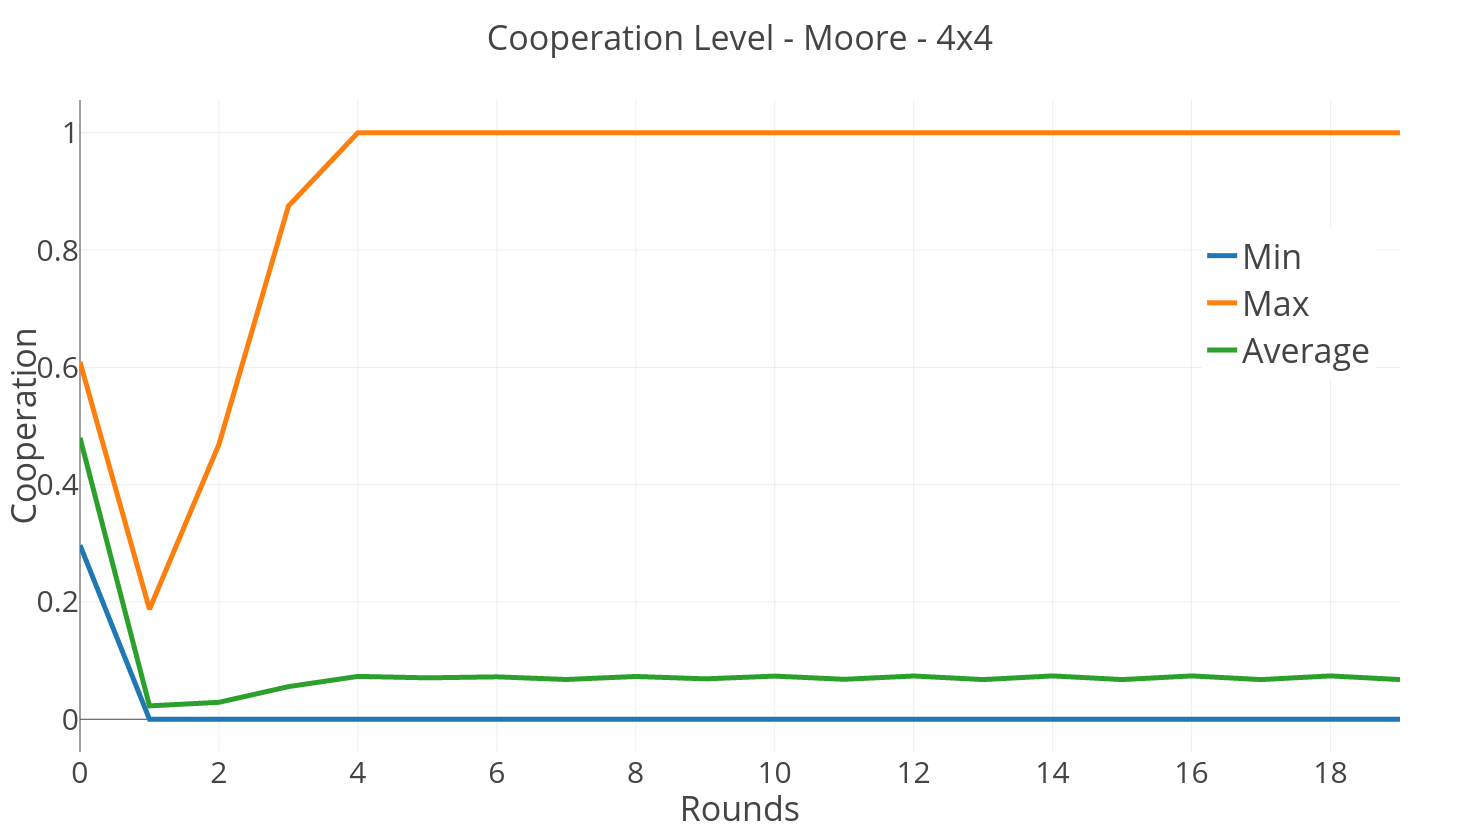
\includegraphics[width=1\linewidth]{PDMoore8x8}
\end{subfigure}

\begin{subfigure}{.75\textwidth}
	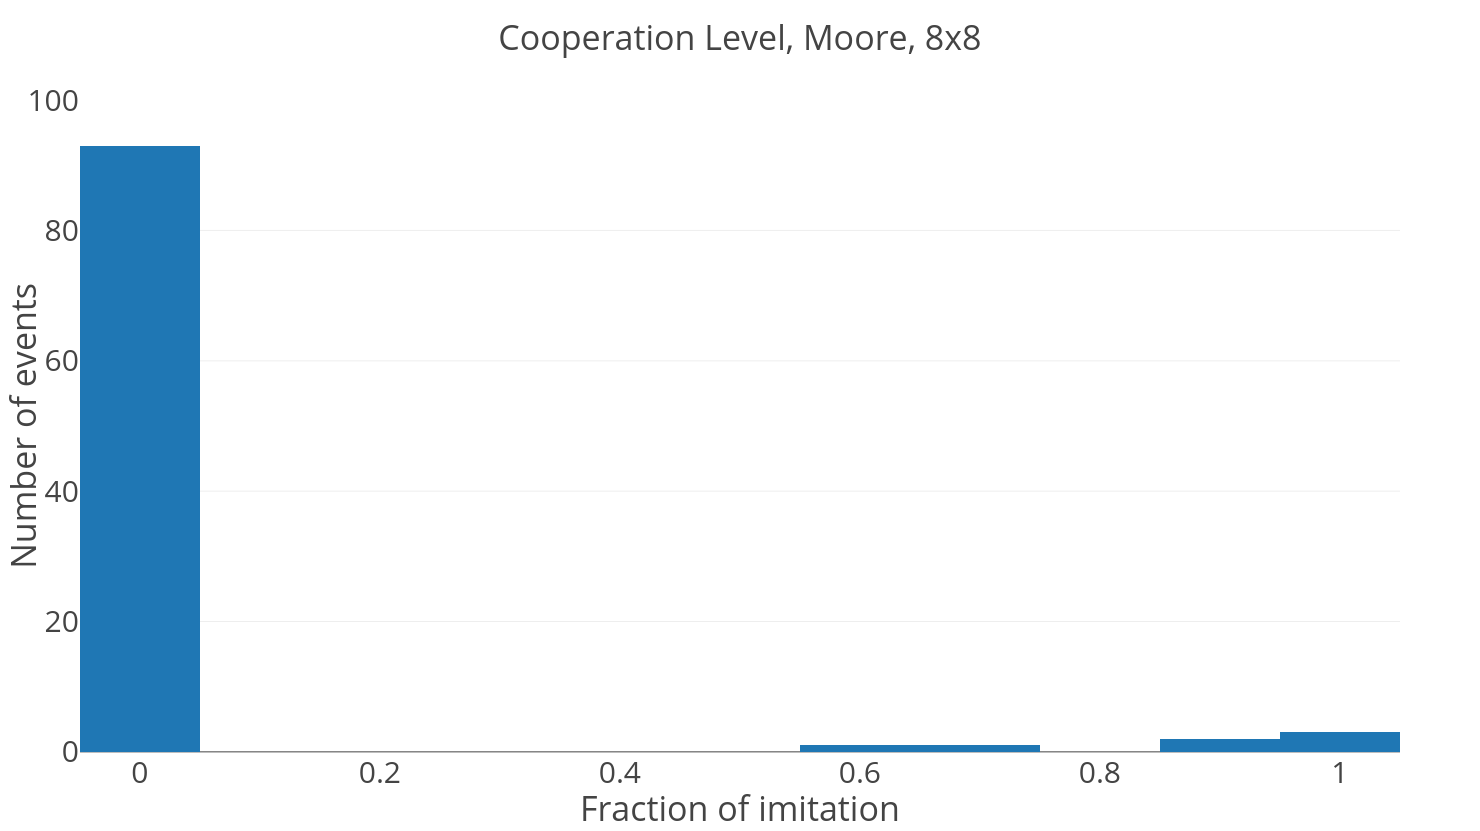
\includegraphics[width=1\linewidth]{PDMoore8x8HG}
\end{subfigure}%
\begin{subfigure}{.25\textwidth}
	mean = $0.0605$
	
	deviation = $0.2251$
\end{subfigure}

\end{figure}

converge at 10, 20 rounds

	From simulating 100 runs we observe that all converge to \textit{defecting}. It is however possible that it converges to a cooperative field, but it requires that we have a sub-matrix of 2x2 with only cooperators and all other players being defectors. This did obviously not happen during one of the simulations.


\newpage

%%%% 12x12
%%%%%%%%%%%%%%%%%%%%%%%%%%%%%%%%%%%%%%%%%
\subsubsection{12x12}
\begin{figure}[H]
\centering
\begin{subfigure}{.16\textwidth}
  \centering
  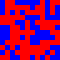
\includegraphics[width=0.9\linewidth]{PRISONERS_DILEMMA_MOORE_12x12_t00}
  \caption{t=0}
\end{subfigure}%
\begin{subfigure}{.16\textwidth}
  \centering
  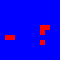
\includegraphics[width=0.9\linewidth]{PRISONERS_DILEMMA_MOORE_12x12_t01}
  \caption{t=1}
\end{subfigure}%
\begin{subfigure}{.16\textwidth}
  \centering
  
\includegraphics[width=0.9\linewidth]{PRISONERS_DILEMMA_MOORE_12x12_t05}
  \caption{t=5}
\end{subfigure}%
\begin{subfigure}{.16\textwidth}
  \centering
  
\includegraphics[width=0.9\linewidth]{PRISONERS_DILEMMA_MOORE_12x12_t10}
  \caption{t=10}
\end{subfigure}%
\begin{subfigure}{.16\textwidth}
  \centering
  
\includegraphics[width=0.9\linewidth]{PRISONERS_DILEMMA_MOORE_12x12_t20}
  \caption{t=20}
\end{subfigure}%
\begin{subfigure}{.16\textwidth}
  \centering
  
\includegraphics[width=0.9\linewidth]{PRISONERS_DILEMMA_MOORE_12x12_t50}
  \caption{t=50}
\end{subfigure}
\caption{Prisoners Dilemma, Moore, 12x12}
\end{figure}


\begin{figure}[H]
\begin{subfigure}{.75\textwidth}
	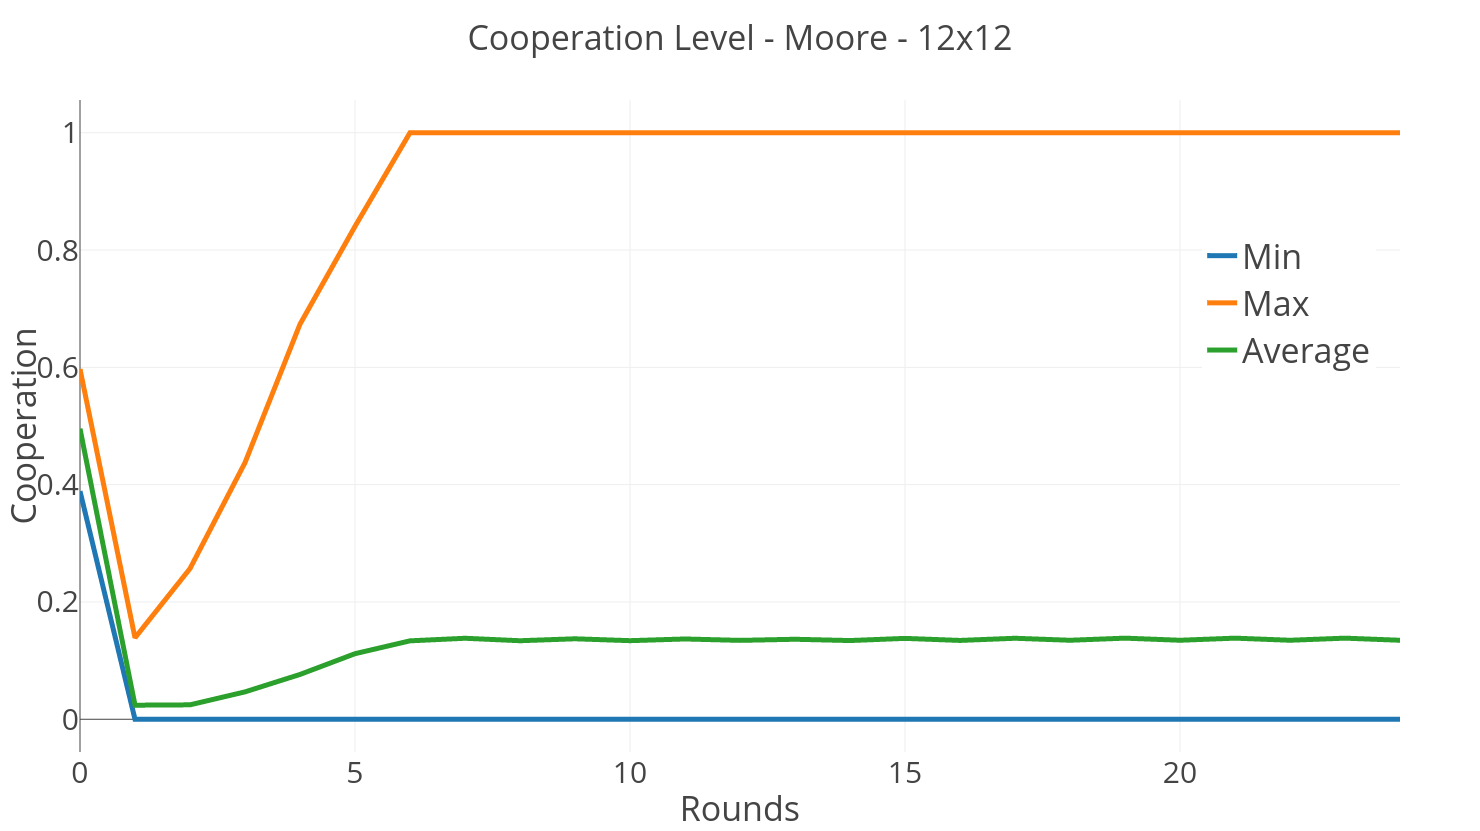
\includegraphics[width=1\linewidth]{PDMoore12x12}
\end{subfigure}

\begin{subfigure}{.75\textwidth}
	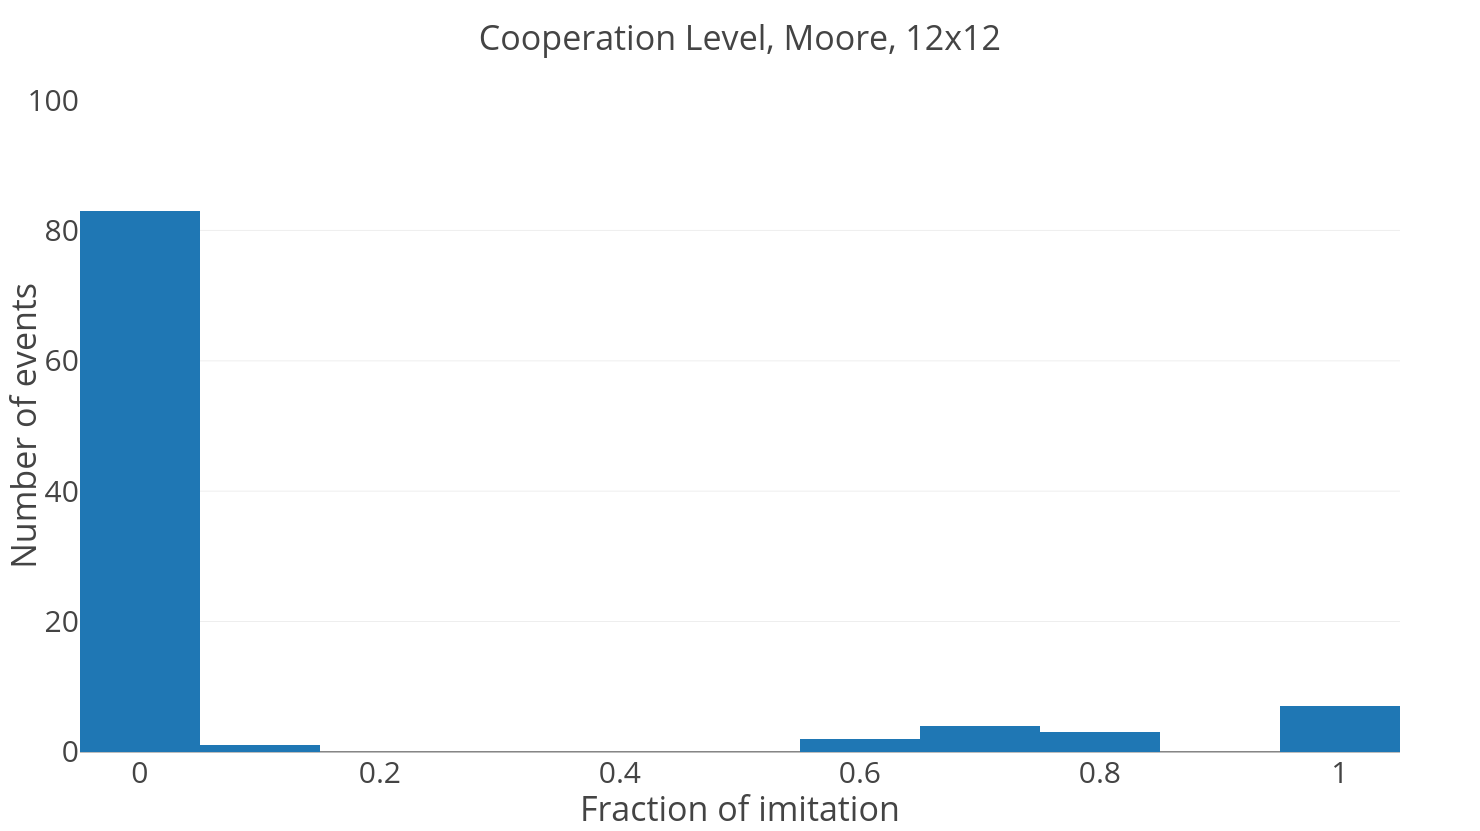
\includegraphics[width=1\linewidth]{PDMoore12x12HG}
\end{subfigure}%
\begin{subfigure}{.25\textwidth}
	mean = $0.1347$
	
	deviation = $0.3115$
\end{subfigure}

\end{figure}

converge at 10, 25 rounds

	From simulating 100 runs we observe that all converge to \textit{defecting}. It is however possible that it converges to a cooperative field, but it requires that we have a sub-matrix of 2x2 with only cooperators and all other players being defectors. This did obviously not happen during one of the simulations.

\newpage

%%%% 20x20
%%%%%%%%%%%%%%%%%%%%%%%%%%%%%%%%%%%%%%%%%
\subsubsection{20x20}
\begin{figure}[H]
\centering
\begin{subfigure}{.16\textwidth}
  \centering
  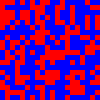
\includegraphics[width=0.9\linewidth]{PRISONERS_DILEMMA_MOORE_20x20_t00}
  \caption{t=0}
\end{subfigure}%
\begin{subfigure}{.16\textwidth}
  \centering
  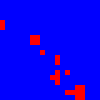
\includegraphics[width=0.9\linewidth]{PRISONERS_DILEMMA_MOORE_20x20_t01}
  \caption{t=1}
\end{subfigure}%
\begin{subfigure}{.16\textwidth}
  \centering
  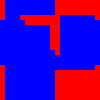
\includegraphics[width=0.9\linewidth]{PRISONERS_DILEMMA_MOORE_20x20_t05}
  \caption{t=5}
\end{subfigure}
\begin{subfigure}{.16\textwidth}
  \centering
  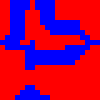
\includegraphics[width=0.9\linewidth]{PRISONERS_DILEMMA_MOORE_20x20_t10}
  \caption{t=10}
\end{subfigure}%
\begin{subfigure}{.16\textwidth}
  \centering
  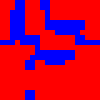
\includegraphics[width=0.9\linewidth]{PRISONERS_DILEMMA_MOORE_20x20_t20}
  \caption{t=20}
\end{subfigure}%
\begin{subfigure}{.16\textwidth}
  \centering
  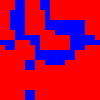
\includegraphics[width=0.9\linewidth]{PRISONERS_DILEMMA_MOORE_20x20_t50}
  \caption{t=50}
\end{subfigure}
\caption{Prisoners Dilemma, Moore, 20x20}
\end{figure}

\begin{figure}[H]
\begin{subfigure}{.75\textwidth}
	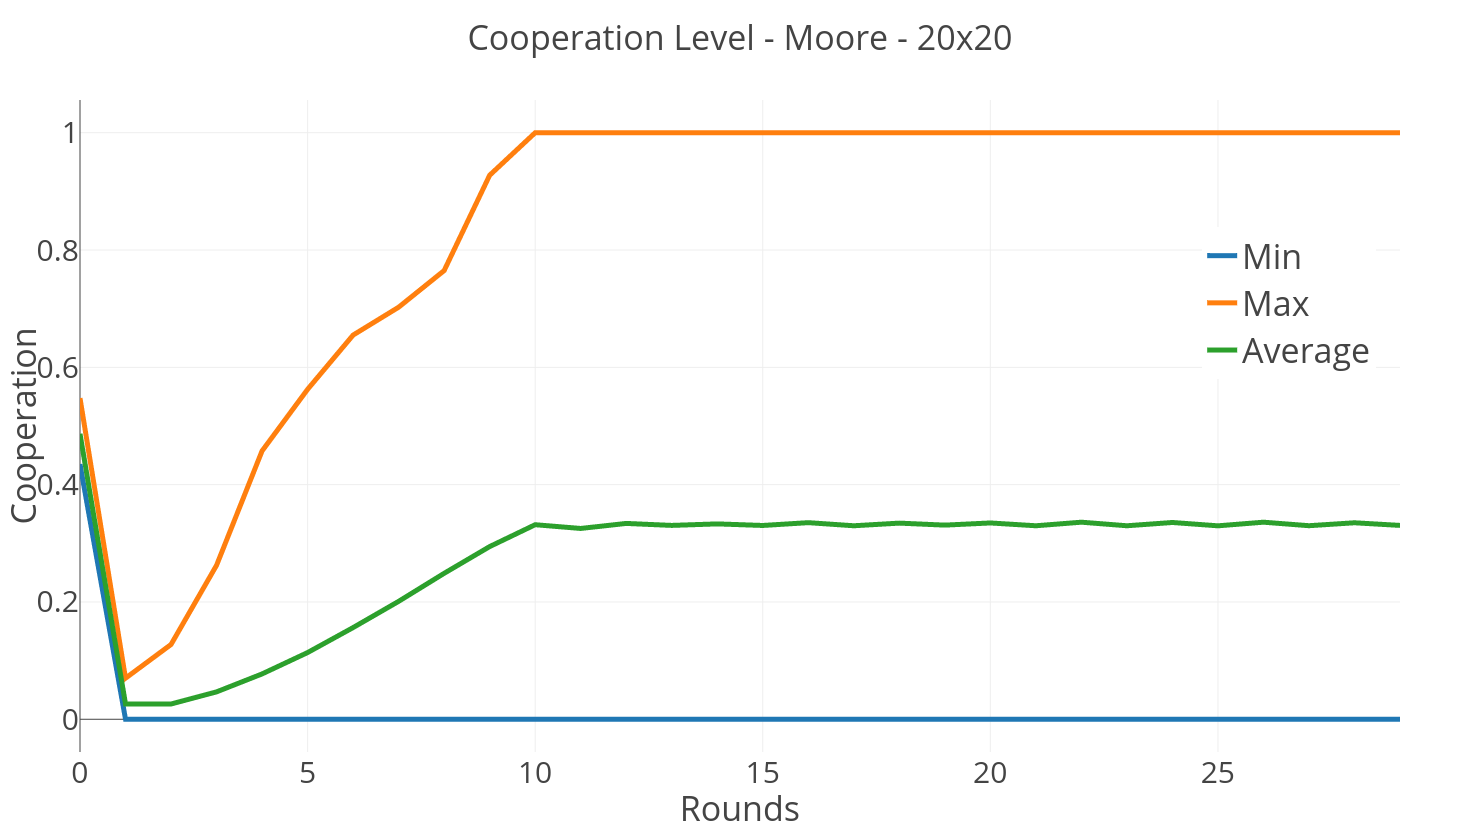
\includegraphics[width=1\linewidth]{PDMoore20x20}
\end{subfigure}

\begin{subfigure}{.75\textwidth}
	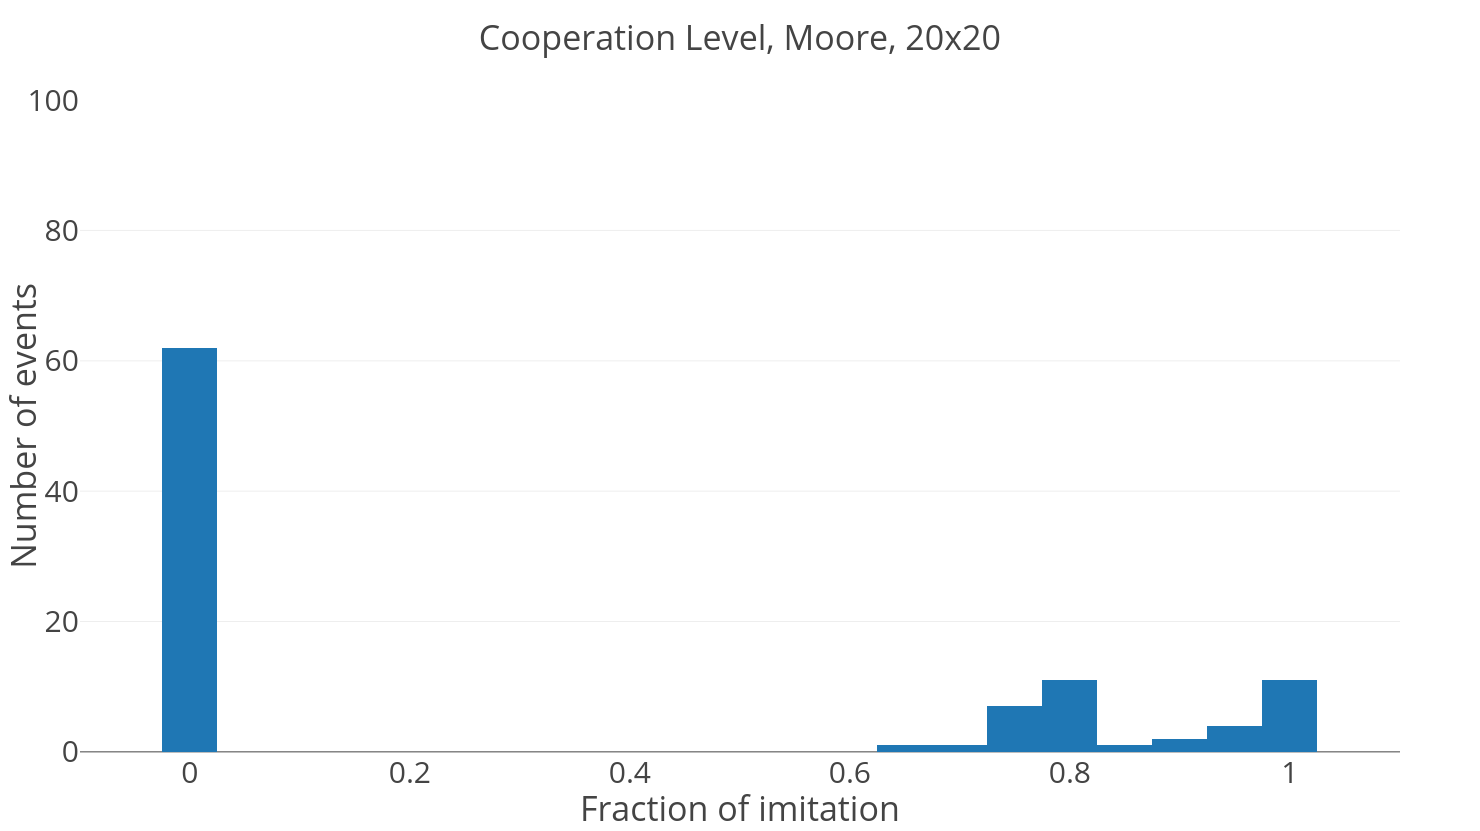
\includegraphics[width=1\linewidth]{PDMoore20x20HG}
\end{subfigure}%
\begin{subfigure}{.25\textwidth}
	mean = $0.3305$
	
	deviation = $0.4262$
\end{subfigure}

\end{figure}

	From simulating 100 runs we observe that all converge to \textit{defecting}. It is however possible that it converges to a cooperative field, but it requires that we have a sub-matrix of 2x2 with only cooperators and all other players being defectors. This did obviously not happen during one of the simulations.


\newpage
%%%% 50x50
%%%%%%%%%%%%%%%%%%%%%%%%%%%%%%%%%%%%%%%%%
\subsubsection{50x50}
\begin{figure}[H]
\centering
\begin{subfigure}{.16\textwidth}
  \centering
  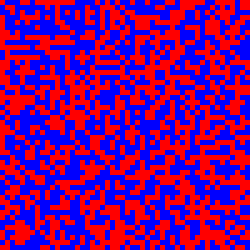
\includegraphics[width=0.9\linewidth]{PRISONERS_DILEMMA_MOORE_50x50_t00}
  \caption{t=0}
\end{subfigure}%
\begin{subfigure}{.16\textwidth}
  \centering
  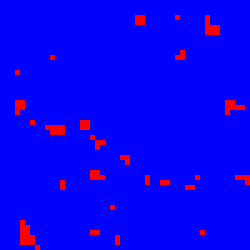
\includegraphics[width=0.9\linewidth]{PRISONERS_DILEMMA_MOORE_50x50_t01}
  \caption{t=1}
\end{subfigure}%
\begin{subfigure}{.16\textwidth}
  \centering
  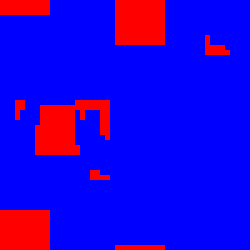
\includegraphics[width=0.9\linewidth]{PRISONERS_DILEMMA_MOORE_50x50_t05}
  \caption{t=5}
\end{subfigure}
\begin{subfigure}{.16\textwidth}
  \centering
  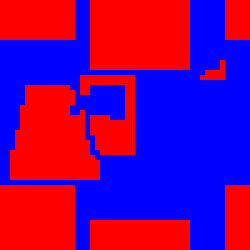
\includegraphics[width=0.9\linewidth]{PRISONERS_DILEMMA_MOORE_50x50_t10}
  \caption{t=10}
\end{subfigure}%
\begin{subfigure}{.16\textwidth}
  \centering
  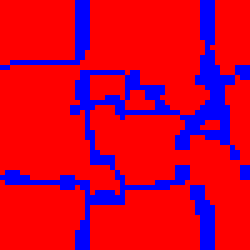
\includegraphics[width=0.9\linewidth]{PRISONERS_DILEMMA_MOORE_50x50_t20}
  \caption{t=20}
\end{subfigure}%
\begin{subfigure}{.16\textwidth}
  \centering
  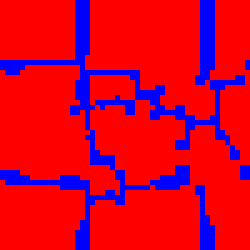
\includegraphics[width=0.9\linewidth]{PRISONERS_DILEMMA_MOORE_50x50_t50}
  \caption{t=50}
\end{subfigure}
\caption{Prisoners Dilemma, Moore, 50x50}
\end{figure}

\begin{figure}[H]
\begin{subfigure}{.75\textwidth}
	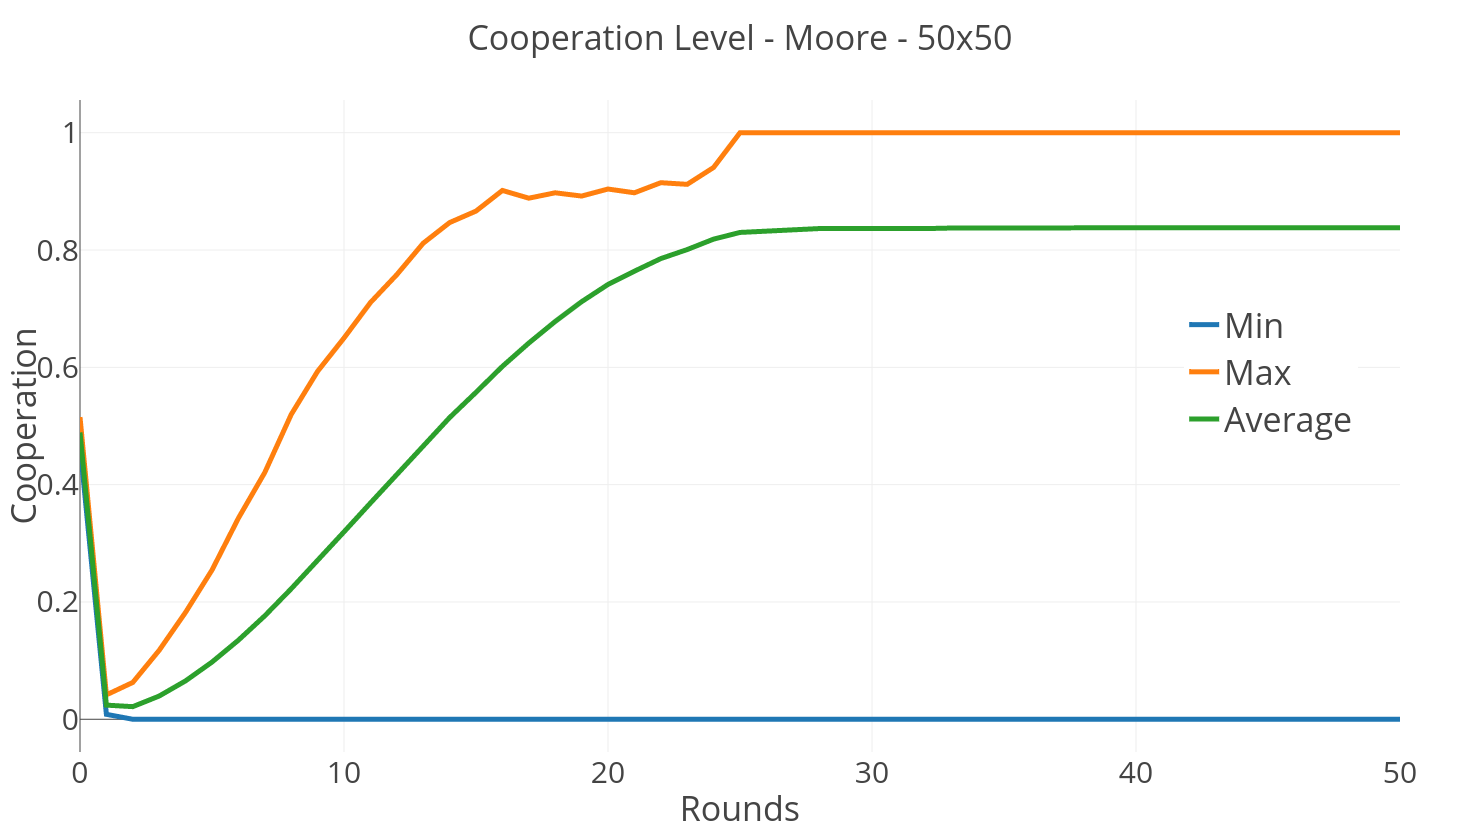
\includegraphics[width=1\linewidth]{PDMoore50x50}
\end{subfigure}

\begin{subfigure}{.75\textwidth}
	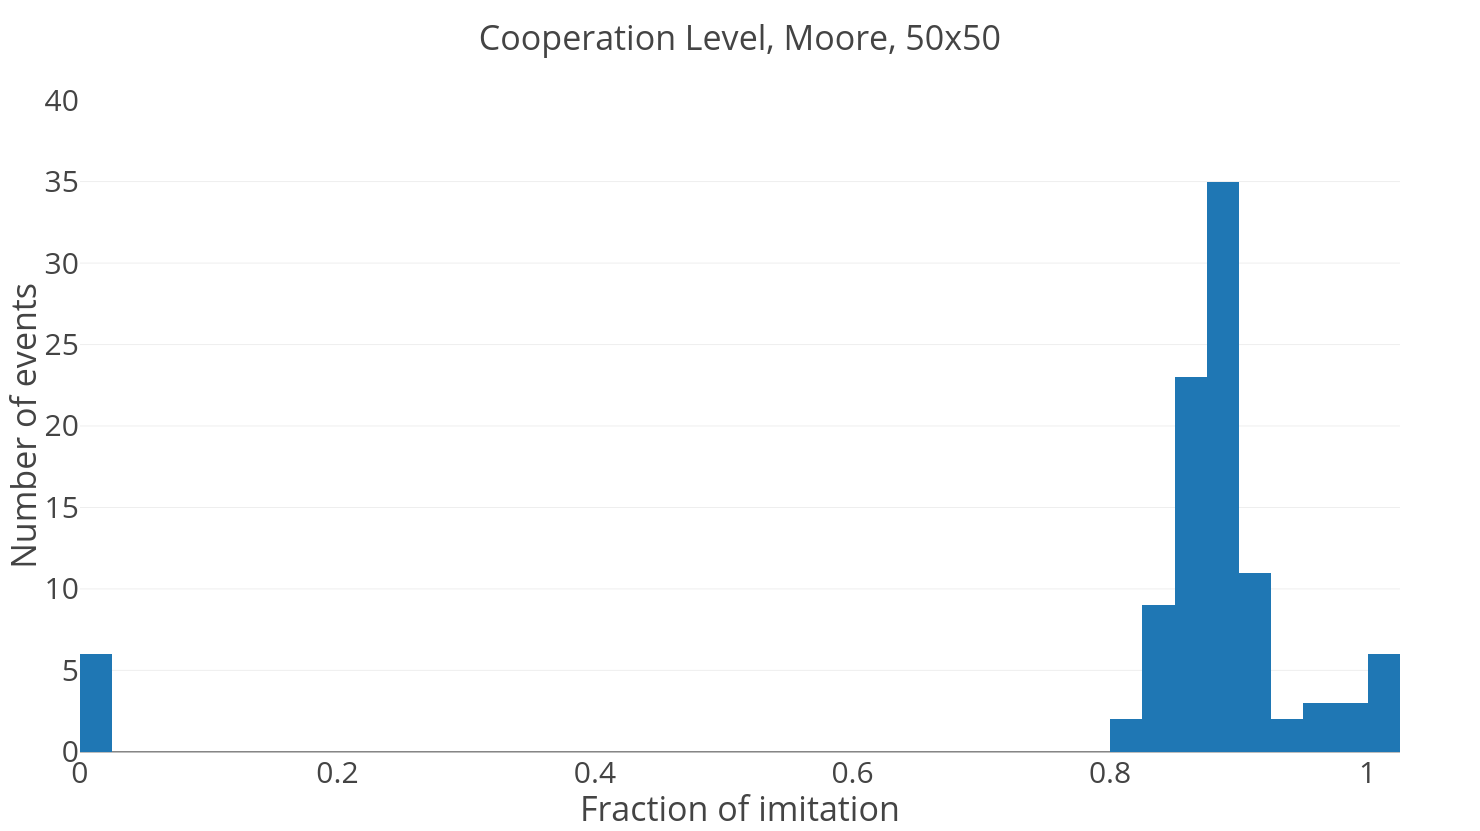
\includegraphics[width=1\linewidth]{PDMoore50x50HG}
\end{subfigure}%
\begin{subfigure}{.25\textwidth}
	mean = $0.8379$
	
	deviation = $0.2165$
\end{subfigure}

\end{figure}

blablabla


%%%%%%%%%%%%%%%%%%%%%%%%%%%%%%%%%%%%%%%%%%%%%%%%
%%%%%%%%%%%%%%%%%%%%%%%%%%%%%%%%%%%%%%%%%%%%%%%%
%%%%%%%%%%%%%%%%%%%%%%%%%%%%%%%%%%%%%%%%%%%%%%%%

\newpage
\section{Part Two}


%%%%%%%%%%%%%%%%%%%%%%%%%%%%%%%%%%%%%%%%%%%%%%%%
%%%%%%%%%%%%%%%%%%%%%%%%%%%%%%%%%%%%%%%%%%%%%%%%
%%%%%%%%%%%%%%%%%%%%%%%%%%%%%%%%%%%%%%%%%%%%%%%%
\newpage
\section{Part Three}

\end{document}